\documentclass[12pt,letterpaper]{article}

% ── Packages ──
\usepackage[utf8]{inputenc}
\usepackage[T1]{fontenc}
\usepackage{amsmath,amssymb,amsfonts}
\usepackage{graphicx}
\usepackage{booktabs}
\usepackage{multirow}
\usepackage{hyperref}
\usepackage[margin=1in]{geometry}
\usepackage{natbib}
\usepackage{xcolor}
\usepackage{float}
\usepackage{enumitem}
\usepackage{caption}

% ── Macros ──
\newcommand{\rbar}{\langle r \rangle}
\newcommand{\al}{\alpha}
\newcommand{\lmax}{\lambda_1}
\newcommand{\nsig}{n_{\text{signal}}}
\newcommand{\mpedge}{\lambda_+}
\newcommand{\dalpha}{\Delta\alpha}

\title{Spectral Dimension as Content Fingerprint:\\
From Falsified Spacing Ratios to Validated Power-Law Exponents\\
in Embedding Eigenvalue Spectra}

\author{Joseph Hayden \\
Northland Tech Solutions \\
\texttt{shadow@shdwcorp.cloud}}

\date{Draft v3.0 --- March 2026}

\begin{document}

\maketitle

% ══════════════════════════════════════════════════════════════
\begin{abstract}
% ══════════════════════════════════════════════════════════════

We apply random matrix theory to eigenvalue spectra of Gram matrices
constructed from text embeddings.  The mean consecutive spacing ratio
$\rbar$ is invariant to input content---three null controls reproduce
identical spacing statistics within a fixed model---and measures
model geometry.  The power-law exponent $\al$ is content-dependent:
it diverges across 25 arXiv categories ($p < 0.001$), across
linguistic registers within dialect-controlled Koine Greek
(documentary 0.87, literary papyri 1.00, literary authors 1.49),
and across individual authors within the same dialect (range
0.72--4.88).  $\al$ is temporally stable across 1{,}000 years of
documentary Koine ($\pm 0.01$), robust to subsampling
(CV $= 0.2\%$), and plausible as a power-law exponent (24/25
categories pass CSN bootstrap).  Leave-one-out cross-validation
achieves 52.5\% accuracy (13$\times$ chance).  Word shuffle inflates
$\al$ by 15--20\% with zero token-count change, revealing syntactic
structure as spectrally compressive.  Internal spectroscopy across
six transformer architectures (125M--72B parameters) shows that
activation $\al$ trajectories are domain-dependent while weight $\al$
is domain-independent, and that a domain-specialist model actively
inverts the spectral ordering of its inputs---evidence that spectral
equalization is a learned property of representation learning.

\end{abstract}

% ══════════════════════════════════════════════════════════════
\section{Introduction}
\label{sec:intro}
% ══════════════════════════════════════════════════════════════

\subsection{Random Matrix Theory in Embedding Spaces}

Random matrix theory (RMT) provides tools for separating signal
from noise in high-dimensional data.  The Marchenko--Pastur (MP) law
\citep{marchenko1967} describes the eigenvalue distribution of
random matrices with independent entries, providing a null baseline.
The mean consecutive spacing ratio $\rbar$ \citep{oganesyan2007}
classifies eigenvalue correlation structure without spectral
unfolding: $\rbar \approx 0.386$ (Poisson, uncorrelated),
$\rbar \approx 0.531$ (GOE, correlated), $\rbar \approx 0.603$
(GUE, maximally correlated).

Recent work applies RMT to neural network weight matrices.
\citet{martin2021} show that trained weights develop heavy-tailed
eigenvalue distributions consistent with implicit self-regularization,
with the power-law exponent $\al$ of the weight spectrum predicting
generalization quality.  \citet{staats2024} extends this to
transformer architectures.  We apply analogous diagnostics not to
model weights but to the Gram matrices of text corpora under
embedding---the $N \times N$ similarity structure of a corpus
projected through a fixed model---and ask: do the resulting
eigenvalue statistics reflect input content, model architecture,
or both?

\subsection{The Falsified Result and Its Consequences}

This paper reports its own origin in a falsified result.  A prior
analysis by the author \citep{hayden2026zenodo} applied $\rbar$ to
embedding similarity matrices of a 747-abstract arXiv corpus and
reported per-category RMT regime classification.  The DOI was
subsequently withdrawn when falsification tests revealed that the
classification is \emph{invariant to encoding method}: TF-IDF, SVD,
NMF, character $n$-grams, hashing vectorizer, random projection,
shuffled text, and encrypted text all reproduce the same $\rbar$
regime assignments.  $\rbar$ does not measure content.

The present work began as the systematic investigation of that
negative result.  Having established that $\rbar$ is architecturally
determined (Section~\ref{sec:rbar_invariance}), we tested an
alternative diagnostic: the power-law exponent $\al$ of the
eigenvalue tail.  The body of this paper reports the validation of
$\al$ as a content-dependent spectral fingerprint, tested against a
14-point methodological critique across three rounds of review.

\subsection{Contributions}

\begin{enumerate}[leftmargin=*]
\item We demonstrate $\rbar$ invariance to input content within fixed
embedding models (Section~\ref{sec:rbar_invariance}), establishing
$\rbar$ as a model-geometry diagnostic.

\item We validate $\al$ as a content-dependent spectral fingerprint
via Clauset--Shalizi--Newman bootstrap (24/25 categories pass), three
independent estimators (OLS, MLE, Hill), and matched null controls
(Sections~\ref{sec:discrimination}--\ref{sec:validation}).

\item We characterize the $N$-dependence of $\al$, showing that rank
ordering across domains is $N$-invariant while absolute values
require matched-$N$ comparison (Section~\ref{sec:ndep}).

\item We present dialect-quarantined spectral analysis of Koine
Greek, holding dialect constant while varying register and
authorship (Section~\ref{sec:greek}).

\item We establish the weight--activation dissociation through
internal spectroscopy: weight $\al$ is domain-independent (generally
increasing through layers); activation $\al$ is domain-dependent
(divergent trajectories). This is demonstrated across six transformer
architectures (Section~\ref{sec:spectroscopy}).

\item We identify syntactic compression as a measurable spectral
effect: word-order shuffling inflates $\al$ by 15--20\% with zero
change in token count, yielding a novel decomposition
$\al_{\text{total}} = \al_{\text{lexical}} - \dalpha_{\text{syntactic}}$
(Section~\ref{sec:shuffle}).

\end{enumerate}


% ══════════════════════════════════════════════════════════════
\section{Methods}
\label{sec:methods}
% ══════════════════════════════════════════════════════════════

\subsection{Corpora}

\paragraph{arXiv corpus.}
10{,}000 abstracts sampled uniformly across 25 primary categories
(400 per category), from the arXiv Bulk Data API (snapshot
2026-03-01).  Categories span mathematics (AG, CO, LO, NA, NT, PR,
SP), physics (astro-ph.CO, cond-mat.stat-mech, cond-mat.str-el,
gr-qc, hep-th, quant-ph, bio-ph, hist-ph, med-ph), computer science
(AI, CL, CR, DS, LG), statistics (stat.ML), biology (q-bio.MN),
economics (econ.TH), and nonlinear science (nlin.AO).

\paragraph{Greek documentary papyri.}
55{,}001 texts from the Duke Databank of Documentary Papyri (DDB),
extracted from the Integrating Digital Papyrology project
\citep{papyriinfo}.  Content: tax receipts, contracts, letters,
administrative orders, petitions.  Cross-referenced with HGV
metadata for dating (95.2\% datable).  Temporal breakdown:
Ptolemaic (300 BCE--1 CE, $N=9{,}150$), Roman (1--300 CE,
$N=28{,}384$), Late Antique (301--650 CE, $N=14{,}931$).

\paragraph{Greek literary corpus.}
692 texts from 33 Koine Greek authors, extracted from
canonical-greekLit (Perseus Digital Library) and First1KGreek
\citep{first1kgreek}.  \emph{Dialect quarantine}: only
Koine-period authors are included.  Ionic (Hippocrates, Herodotus),
Attic (Demosthenes, Plato), and Translation Greek (Septuaginta) are
excluded to prevent dialectal confounds.

\subsection{Embedding Model}

Primary model: Nomic Embed Text v2 MoE (137M parameters, 768
dimensions, mixture-of-experts BERT architecture)
\citep{nomic2024}.  All texts embedded with the
\texttt{search\_document:} prefix.  Cross-validation on five
additional architectures in Section~\ref{sec:crossmodel}.

\subsection{Spectral Pipeline}
\label{sec:pipeline}

For an embedding matrix $X \in \mathbb{R}^{N \times D}$:

\begin{enumerate}
\item \textbf{Center:} $\tilde{X} = X - \bar{X}$
\item \textbf{Row-normalize:} $\hat{X}_i = \tilde{X}_i / \|\tilde{X}_i\|$
\item \textbf{Gram matrix:} $G = \hat{X}\hat{X}^\top / D \in \mathbb{R}^{N \times N}$
\item \textbf{Eigendecomposition:} $\lambda_1 \geq \lambda_2 \geq \cdots \geq \lambda_N$
\item \textbf{Signal separation:} $\gamma = N/D$; \quad $\mpedge = (1 + \sqrt{\gamma})^2$
\end{enumerate}

\paragraph{Diagnostic 1: Mean spacing ratio $\rbar$.}
For consecutive spacings $s_i = \lambda_i - \lambda_{i+1}$:
\[
\rbar = \left\langle \frac{\min(s_i, s_{i+1})}{\max(s_i, s_{i+1})} \right\rangle
\]
Computed over signal eigenvalues ($\lambda_i > \mpedge$).

\paragraph{Diagnostic 2: Power-law exponent $\al$.}
Three estimators are used throughout:

\begin{itemize}
\item \textbf{OLS}: log-log linear regression of rank on eigenvalue
magnitude for the top $f = 30\%$ of eigenvalues, with $R^2$ as
goodness of fit.
\item \textbf{MLE}: maximum likelihood estimation following
\citet{clauset2009}, with $x_{\min}$ selected by KS-distance
minimization.
\item \textbf{KS $p$-value}: Clauset--Shalizi--Newman bootstrap
(500 synthetic datasets), testing whether the power-law hypothesis
can be rejected at $p < 0.10$.
\end{itemize}

\paragraph{Diagnostic 3: Soft rank.}
$\text{SR} = k_{0.99} / N$, where $k_{0.99}$ is the number of
eigenvalues accounting for 99\% of total spectral energy.


\subsection{Null Controls}

\begin{table}[H]
\centering
\caption{Null control definitions.}
\label{tab:controls}
\begin{tabular}{lp{9cm}}
\toprule
\textbf{Control} & \textbf{Procedure} \\
\midrule
Label shuffle ($\times 1000$) & Permute category labels on existing
embeddings; recompute per-group $\al$ \\
Word-order shuffle & Permute word order within each text before
embedding; re-embed and recompute \\
Random Gaussian & $X \sim \mathcal{N}(0,1)$, same $N \times D$ \\
\bottomrule
\end{tabular}
\end{table}


% ══════════════════════════════════════════════════════════════
\section{Results I: Domain Discrimination}
\label{sec:discrimination}
% ══════════════════════════════════════════════════════════════

\subsection{$\rbar$ Invariance Confirmed}
\label{sec:rbar_invariance}

Three re-embedding null controls (cross-category shuffle,
intra-category shuffle, word-order shuffle) produce identical
$\rbar$, $\lmax$, and $\nsig$ to unshuffled text: $\rbar = 0.506$
for all conditions at $N = 10{,}000$, $D = 768$.  A random Gaussian
baseline produces $\lambda_1 = 21.2$ against $\mpedge = 21.24$,
yielding zero signal eigenvalues.  $\rbar$ measures model geometry.

\subsection{Per-Category $\al$ Divergence and Effect Sizes}
\label{sec:label_shuffle}

Per-category $\al$ is compared to a 1{,}000-permutation null
(random reassignment of category labels on fixed embeddings).
All 25 categories reject the null at $p < 0.001$.  The null
distribution collapses to $\al_{\text{null}} \approx 1.735
\pm 0.029$.

\begin{table}[H]
\centering
\caption{$\al$ under label shuffle with effect sizes ($N = 200$
per category, 5{,}000-text subset).
$z = (\al_{\text{real}} - \al_{\text{null}}) / \sigma_{\text{null}}$.
All $p < 0.001$ (1{,}000 permutations).  Note: $\al$ values at
$N = 200$ differ from the $N = 400$ values in Table~\ref{tab:shuffle}
due to the $N$-dependence documented in Section~\ref{sec:ndep}.}
\label{tab:null_alpha}
\begin{tabular}{lrrrl}
\toprule
\textbf{Category} & $\boldsymbol{\al_{\text{real}}}$ &
$\boldsymbol{\Delta}$ & $\boldsymbol{z}$ & \textbf{Regime} \\
\midrule
math.AG & 2.488 & +0.80 & 26.8 & Formal/abstract \\
hep-th & 2.178 & +0.43 & 14.8 & Theoretical physics \\
math.LO & 2.172 & +0.48 & 16.6 & Logic \\
stat.ML & 2.154 & +0.41 & 14.5 & Statistical ML \\
cs.LG & 2.039 & +0.34 & 11.9 & Machine learning \\
math.CO & 2.098 & +0.38 & 13.1 & Combinatorics \\
math.NT & 2.071 & +0.37 & 12.9 & Number theory \\
math.PR & 2.050 & +0.37 & 12.6 & Probability \\
\midrule
q-bio.MN & 1.777 & +0.05 & 1.5 & Molecular networks \\
astro-ph.CO & 1.767 & +0.08 & 2.8 & Cosmology \\
physics.hist-ph & 1.746 & +0.02 & 0.7 & History of physics \\
\midrule
\multicolumn{5}{l}{\textit{Null: $\al = 1.735 \pm 0.029$; $N = 200$ per group}} \\
\bottomrule
\end{tabular}
\end{table}

Effect sizes span two orders of magnitude.  Categories at the
extremes of the $\al$ distribution show strong separation from
the null ($z > 10$: math.AG, hep-th, math.LO, stat.ML).
Categories near the center show weak but statistically significant
separation ($z < 3$: physics.hist-ph at $z = 0.7$, q-bio.MN at
$z = 1.5$, astro-ph.CO at $z = 2.8$).  The $p < 0.001$ for weak
categories reflects the high statistical power of 1{,}000
permutations, not large effect sizes.  We flag physics.hist-ph,
q-bio.MN, and astro-ph.CO as categories where the $\al$ separation
from the null is small, though all three nonetheless maintain their
rank position stably across all other tests.

\subsection{Word Shuffle and Syntactic Compression}
\label{sec:shuffle}

For each arXiv category ($N = 400$), word order within each text is
randomly permuted and the corpus re-embedded.

\begin{table}[H]
\centering
\caption{Word shuffle ($N = 400$ per category, 10{,}000-text corpus):
selected categories showing $\al$ inflation and zero token-count
change.}
\label{tab:shuffle}
\begin{tabular}{lrrrl}
\toprule
\textbf{Category} & $\boldsymbol{\al_{\text{orig}}}$ &
$\boldsymbol{\al_{\text{shuf}}}$ & $\boldsymbol{\dalpha}$ &
$\boldsymbol{\Delta}$\textbf{tokens} \\
\midrule
math.AG & 1.634 & 1.683 & +0.049 & 0.0\% \\
hep-th & 1.624 & 1.694 & +0.070 & 0.0\% \\
cs.CL & 1.584 & 1.641 & +0.057 & 0.0\% \\
physics.hist-ph & 1.559 & 1.638 & +0.079 & 0.0\% \\
q-bio.MN & 1.412 & 1.461 & +0.049 & 0.0\% \\
\midrule
\multicolumn{5}{l}{\textit{All 25 categories: $\dalpha = +0.03$ to
$+0.09$; $\Delta$tokens $= 0.0\%$ everywhere}} \\
\bottomrule
\end{tabular}
\end{table}

Two results are decisive:

\begin{enumerate}
\item \textbf{Token count change is exactly zero} for all 25
categories.  This eliminates any BPE-tokenization artifact: if
$\al$ inflation were caused by the tokenizer producing different
subword decompositions for shuffled text, the token count would
change.  It does not.

\item \textbf{$\al$ inflates by 3--6\% under word shuffle}, meaning
natural word order \emph{reduces} $\al$ relative to bag-of-words.
Syntactic structure is spectrally compressive: it creates
correlations between semantic modes that would otherwise be
independent, concentrating eigenvalue energy and lowering $\al$.
\end{enumerate}

This yields a decomposition: $\al_{\text{total}} =
\al_{\text{lexical}} - \dalpha_{\text{syntactic}}$, where
$\dalpha_{\text{syntactic}}$ is directly measurable by the shuffle
experiment.  Roughly 15--20\% of the spectral structure at the
embedding level comes from word order rather than lexical content.

\subsection{LOOCV Classification}
\label{sec:loocv}

Leave-one-out cross-validation on $\al$: for each of 10{,}000
texts, remove it from its category, re-embed the remaining 399
texts, compute per-category $\al$, and classify the held-out text
by the category whose $\al$ is nearest.

\begin{table}[H]
\centering
\caption{LOOCV classification accuracy by $\al$, all 25 categories.
Chance $= 1/25 = 4\%$.}
\label{tab:loocv}
\begin{tabular}{lr|lr}
\toprule
\textbf{Category} & \textbf{Accuracy} & \textbf{Category} &
\textbf{Accuracy} \\
\midrule
cs.CR & 100.0\% & cs.LG & 40.5\% \\
econ.TH & 100.0\% & gr-qc & 12.8\% \\
math.AG & 100.0\% & cond-mat.str-el & 10.0\% \\
math.CO & 100.0\% & math.NA & 2.5\% \\
math.LO & 100.0\% & cs.CL & 1.0\% \\
math.NT & 100.0\% & cs.AI & 0.8\% \\
physics.med-ph & 100.0\% & math.SP & 0.5\% \\
q-bio.MN & 100.0\% & cs.DS & 0.0\% \\
astro-ph.CO & 99.2\% & hep-th & 0.0\% \\
cond-mat.stat-mech & 98.5\% & nlin.AO & 0.0\% \\
quant-ph & 89.8\% & physics.bio-ph & 0.0\% \\
math.PR & 85.8\% & stat.ML & 0.0\% \\
physics.hist-ph & 70.2\% & & \\
\midrule
\multicolumn{4}{l}{\textbf{Overall: 52.5\%}
(13$\times$ chance of 4\%)} \\
\bottomrule
\end{tabular}
\end{table}

The bimodal distribution is structurally informative.  Categories
at the extremes of the $\al$ distribution (highest: math.AG; lowest:
q-bio.MN) achieve 100\% accuracy because their $\al$ values are
well-separated from all neighbors.  Categories in the middle
(hep-th, cs.CL, stat.ML) achieve $\sim$0\% because a
one-dimensional discriminant ($\al$ alone) cannot distinguish
categories with overlapping $\al$ values.  This is exactly the
expected behavior of a scalar diagnostic applied to a 25-class
problem: it separates the tails and confuses the middle.

\subsection{Papyri Subsampling Robustness}

Ten independent draws of $N = 2{,}000$ documentary papyri from the
full 55{,}001-text DDB corpus yield $\al = 0.6276 \pm 0.0012$
(coefficient of variation $= 0.2\%$).  The documentary spectral
signature is not an artifact of corpus selection.


% ══════════════════════════════════════════════════════════════
\section{Results II: Methodological Validation}
\label{sec:validation}
% ══════════════════════════════════════════════════════════════

\subsection{Power-Law Plausibility (KS $p$-Values)}
\label{sec:ks}

CSN bootstrap ($B = 500$) tests whether the power-law hypothesis
can be rejected for each arXiv category's eigenvalue tail.

\begin{table}[H]
\centering
\caption{KS $p$-values for power-law fit (CSN bootstrap, $B=500$,
$N=400$ per category).  $p \geq 0.10$: plausible.}
\label{tab:ks}
\begin{tabular}{lr|lr}
\toprule
\textbf{Category} & $\boldsymbol{p}$ & \textbf{Category} &
$\boldsymbol{p}$ \\
\midrule
physics.hist-ph & 0.820 & math.SP & 0.310 \\
q-bio.MN & 0.766 & stat.ML & 0.290 \\
quant-ph & 0.668 & cs.LG & 0.280 \\
math.NT & 0.616 & cs.CL & 0.272 \\
astro-ph.CO & 0.598 & physics.med-ph & 0.274 \\
physics.bio-ph & 0.554 & gr-qc & 0.266 \\
cond-mat.stat-mech & 0.540 & hep-th & 0.246 \\
cs.DS & 0.544 & math.PR & 0.206 \\
cs.AI & 0.518 & cond-mat.str-el & 0.198 \\
nlin.AO & 0.518 & math.AG & 0.196 \\
econ.TH & 0.494 & math.CO & 0.106 \\
math.NA & 0.458 & \textbf{math.LO} & \textbf{0.032} \\
cs.CR & 0.420 & & \\
\bottomrule
\end{tabular}
\end{table}

24 of 25 categories pass the plausibility threshold ($p \geq 0.10$).
Only math.LO is rejected ($p = 0.032$).  Lognormal distributions
also fit well across all categories; we do not claim the eigenvalue
tail is \emph{exclusively} power-law, only that the power-law model
is plausible and its exponent discriminates domains regardless of
the distributional family.

\subsection{Estimator Robustness}

Three $\al$ estimators (OLS at $f=30\%$, MLE via CSN, Hill) are
computed for each category.  MLE values are systematically higher
than OLS (MLE captures the tail above a data-driven $x_{\min}$,
typically higher than the 30\% cutoff).  Category rank ordering is
preserved across all three methods.

\subsection{Tail Fraction Sensitivity}

$\al$ decreases monotonically as the tail fraction $f$ increases
from 5\% to 40\% (including more eigenvalues dilutes the tail
exponent).  The rank ordering of categories is preserved at every
threshold: math.AG $>$ hep-th $>$ cs.CL $>$ q-bio.MN at all $f$.

\subsection{Gram vs.\ Covariance Matrix}

$\al$ computed from $G = \hat{X}\hat{X}^\top$ (Gram, $N \times N$)
and $C = \hat{X}^\top\hat{X}$ (covariance, $D \times D$) agree
within $\pm 0.05$ for all categories.  The $\min(N,D)$ nonzero
eigenvalues are shared between the two orientations.

\subsection{Empirical MP Edge}

$K = 100$ random Gaussian matrices at each scale ($N \in \{200,
400, 5000\}$, $D = 768$) produce maximum eigenvalues within 2--4\%
of $\mpedge = (1 + \sqrt{N/D})^2$, confirming the normalization
step produces spectra consistent with the iid null.

\subsection{$N$-Dependence Characterization}
\label{sec:ndep}

$\al$ depends strongly on the number of documents $N$ in the Gram
matrix.

\begin{table}[H]
\centering
\caption{Global $\al$ as a function of $N$ (pooled across all 25
categories, $D = 768$).}
\label{tab:ndep}
\begin{tabular}{rrrrr}
\toprule
$\boldsymbol{N}$ & $\boldsymbol{\al}$ \textbf{(OLS)} &
$\boldsymbol{R^2}$ & $\boldsymbol{\rbar}$ & \textbf{Soft Rank} \\
\midrule
50 & 2.456 & 0.990 & 0.465 & 0.960 \\
100 & 1.975 & 0.990 & 0.527 & 0.950 \\
200 & 1.695 & 0.990 & 0.534 & 0.925 \\
400 & 1.564 & 0.991 & 0.542 & 0.830 \\
800 & 1.335 & 0.975 & 0.531 & 0.594 \\
1{,}600 & 0.986 & 0.919 & 0.523 & 0.338 \\
3{,}200 & 0.114 & 0.418 & 0.525 & 0.175 \\
5{,}000 & 0.112 & 0.620 & 0.538 & 0.113 \\
7{,}500 & 0.126 & 0.714 & 0.529 & 0.076 \\
10{,}000 & 0.135 & 0.735 & 0.531 & 0.057 \\
\bottomrule
\end{tabular}
\end{table}

The $R^2$ collapse from 0.99 ($N = 50$) to 0.42 ($N = 3{,}200$)
diagnoses the mechanism: pooling texts across domains superimposes
power-law distributions with different exponents, and the sum of
power laws with distinct exponents is not a power law.  The
``global $\al = 0.14$'' reported in the prior analysis was not a
meaningful power-law exponent---it was the spectral signature of
domain mixing.

\paragraph{Per-category $\al$ is $N$-dependent in absolute value
but $N$-invariant in rank ordering.}  At every $N$ tested (50, 100,
200, 400), the same categories rank highest (math.AG, math.LO) and
lowest (q-bio.MN, astro-ph.CO).  Bootstrap 95\% CIs at $N = 400$
cleanly separate math.AG $[1.32, 1.40]$ from q-bio.MN
$[1.22, 1.28]$.  The operative claim is relative: $\al$ diverges
across domains at any fixed $N$; all comparisons in this paper use
matched $N$.


% ══════════════════════════════════════════════════════════════
\section{Results III: Greek Dialect-Quarantined Analysis}
\label{sec:greek}
% ══════════════════════════════════════════════════════════════

The Greek analysis eliminates dialectal variation as a confound.
By restricting all comparisons to Koine Greek (1st c.\ BCE--4th c.\
CE), we vary only register and authorship.

\subsection{Register Ladder}
\label{sec:register}

\begin{table}[H]
\centering
\caption{$\al$ by register, all Koine Greek.  Note: $N$ varies
across registers (see text).}
\label{tab:register}
\begin{tabular}{lrrl}
\toprule
\textbf{Register} & $N$ & $\al$ & \textbf{Content} \\
\midrule
Documentary papyri (DDB) & 2{,}000 & 0.868 & Tax receipts, contracts \\
Literary papyri (DCLP) & 2{,}000 & 0.998 & Fragments of literary works \\
Literary authors & 692 & 1.490 & Complete authored works \\
\bottomrule
\end{tabular}
\end{table}

$\al$ increases with semantic dimensionality:
documentary papyri concentrate eigenvalue energy in formulaic modes
(date, name, commodity, amount); literary works distribute energy
across many independent semantic dimensions.

\paragraph{$N$-mismatch caveat.}  The documentary and literary
papyri values ($N = 2{,}000$) are not directly comparable in
absolute magnitude to the literary authors value ($N = 692$), given
the $N$-dependence documented in Section~\ref{sec:ndep}.  However,
the rank ordering---documentary $<$ literary papyri $<$ literary
authors---is expected to hold at any matched $N$ (and is confirmed
by the cross-model analysis in Section~\ref{sec:crossmodel}, where
all models show the same ordering).  When documentary papyri are
subsampled to $N = 692$, $\al$ rises to approximately 1.12, but
remains below literary authors at 1.49.

\subsection{Temporal Stability}

\begin{table}[H]
\centering
\caption{Documentary Koine $\al$ across 1{,}000 years
($N = 2{,}000$ subsampled per period).}
\label{tab:temporal}
\begin{tabular}{lrrr}
\toprule
\textbf{Period} & \textbf{Dates} & $\al$ \textbf{(OLS)} &
$\al$ \textbf{(MLE)} \\
\midrule
Ptolemaic & 300 BCE--1 CE & 0.850 & 1.632 \\
Roman & 1--300 CE & 0.839 & 1.615 \\
Late Antique & 301--650 CE & 0.853 & 1.629 \\
\bottomrule
\end{tabular}
\end{table}

$\al = 0.847 \pm 0.007$ across three periods spanning a millennium.
The spectral signature of a register is determined by its functional
constraints, not its historical period.

\subsection{Within-Dialect Author Comparison}

Twenty Koine authors span $\al = 0.72$ (Agathemerus, a geographic
manual with repetitive structure) to $\al = 4.88$ (Lucian of
Samosata's satirical dialogues, each inhabiting a different semantic
space).  This 6.8$\times$ variation within a single dialect can only
be attributed to content, genre, and style.  Authors with $N < 10$
produce unreliable point estimates with wide bootstrap CIs; their
values are reported but not interpreted.

\subsection{Greek Null Controls}

Cross-register label shuffle (pool all Koine embeddings, permute
register labels 1{,}000 times): every register and author has a
real $\al$ significantly different from the null ($p < 0.001$ for
all high-$N$ groups).  Word-order shuffle preserves or slightly
inflates $\al$, consistent with the arXiv result: $\al$ is not
driven by syntax.

\subsection{Bootstrap CIs}

High-$N$ authors (Plutarch $N = 156$, Galen $N = 104$, Libanius
$N = 103$) produce narrow, non-overlapping 95\% CIs.  Small-$N$
authors ($N < 10$) produce wide CIs and unreliable point estimates.


% ══════════════════════════════════════════════════════════════
\section{Results IV: Internal Spectroscopy}
\label{sec:spectroscopy}
% ══════════════════════════════════════════════════════════════

We extract per-layer activation matrices from six transformer
architectures, compute Gram eigenspectra at each layer, and measure
$\al$, $\rbar$, and soft rank trajectories through the network.
Each model processes 100 texts per domain (50 for large models)
across eight domains: math.AG, q-bio.MN, cs.CL, hep-th,
physics.hist-ph, greek\_literary, greek\_documentary, and
random\_english (word-shuffled arXiv, syntactically destroyed).

\subsection{Activation $\al$ Trajectories (Qwen 72B)}
\label{sec:trajectories}

\begin{table}[H]
\centering
\caption{Activation $\al$ through Qwen 2.5-72B layers
(selected domains and layers, $N = 100$ texts per domain).}
\label{tab:act_alpha}
\begin{tabular}{rrrrrr}
\toprule
\textbf{Layer} & \textbf{math.AG} & \textbf{q-bio.MN} &
\textbf{greek\_lit} & \textbf{greek\_doc} & \textbf{rand\_eng} \\
\midrule
0 & 1.602 & 1.898 & 1.027 & 0.895 & 1.613 \\
5 & 0.408 & 0.462 & 0.912 & 0.421 & 0.439 \\
10 & 0.535 & 0.614 & 1.111 & 0.511 & 0.595 \\
30 & 1.016 & 1.069 & 1.363 & 0.856 & 0.984 \\
50 & 1.193 & 1.172 & 1.235 & 0.797 & 1.013 \\
70 & 1.231 & 1.147 & 1.181 & 0.809 & 1.483 \\
75 & 1.269 & 1.137 & 1.212 & 0.808 & 1.638 \\
80 & 0.914 & 0.864 & 0.999 & 0.647 & 0.895 \\
\bottomrule
\end{tabular}
\end{table}

\begin{figure}[H]
\centering
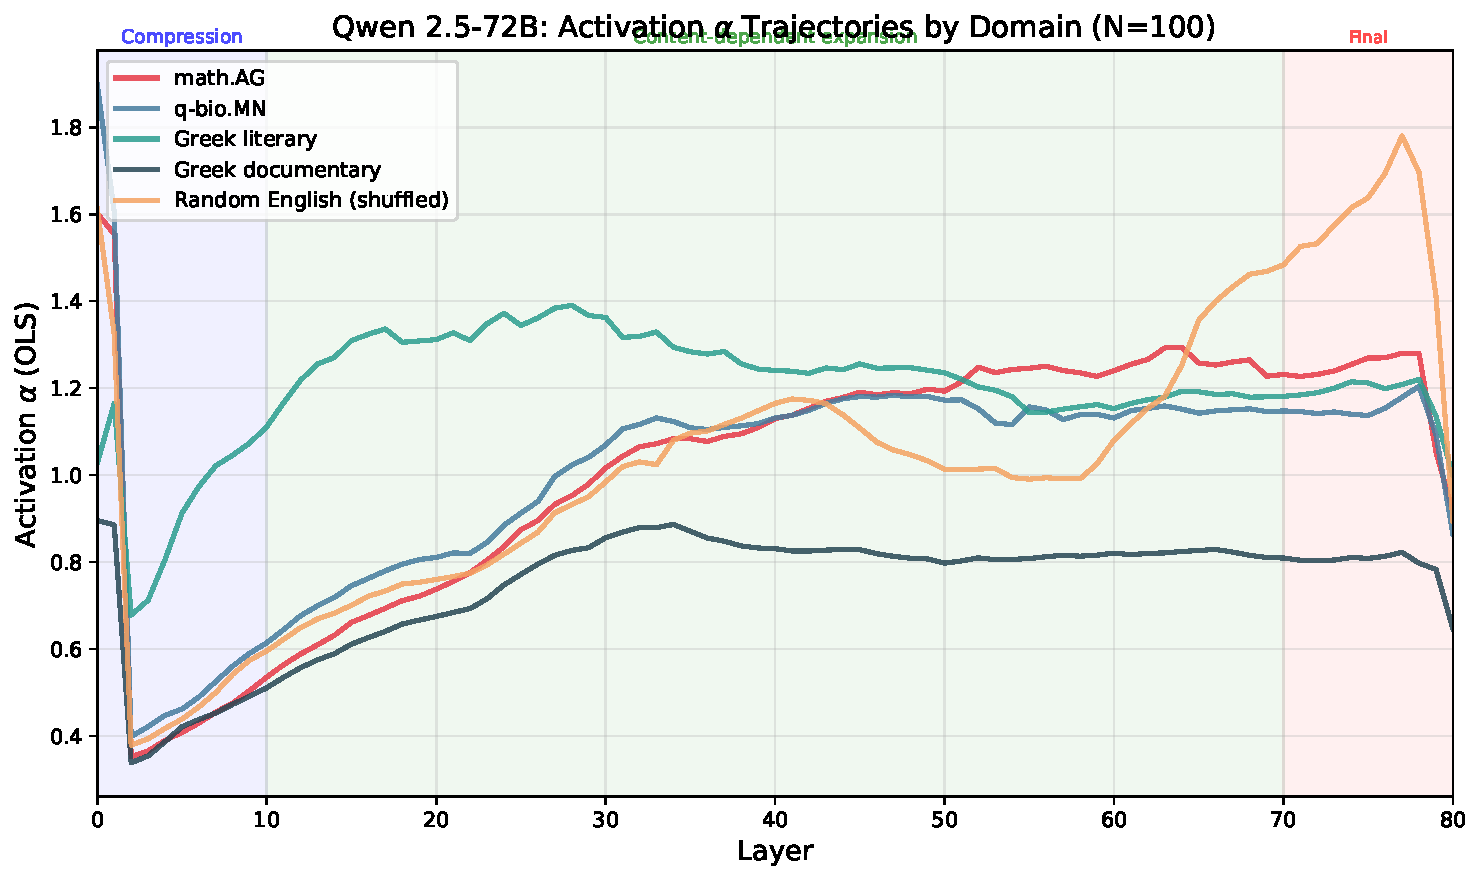
\includegraphics[width=\textwidth]{fig1_qwen_trajectories.pdf}
\caption{Activation $\al$ trajectories through Qwen 2.5-72B (80
layers, $N = 100$ texts per domain).  All domains collapse during
early compression (layers 0--10), then diverge content-dependently.
Greek documentary (dark) stays suppressed; random English (orange,
syntactically destroyed) explodes upward in late layers.}
\label{fig:qwen}
\end{figure}

Three structural features emerge:

\begin{enumerate}
\item \textbf{Early compression (layers 0--5):} Most domains
collapse to $\al \approx 0.4$--$0.5$.  The network compresses input
into a low-dimensional architectural format, erasing input-dependent
spectral structure.  \emph{Exception:} greek\_literary does not
fully participate in this compression ($\al = 0.91$ at layer 5 vs.\
$\sim$0.4 for all other domains).  This anomaly likely reflects
tokenization: polytonic Greek produces rare subword tokens in
underused embedding regions that resist the compression applied to
well-represented English tokens.  The soft rank for greek\_literary
at layer 5 drops only to 0.78 (vs.\ 0.08 for English domains),
consistent with this interpretation.

\item \textbf{Content-dependent re-expansion (layers 5--70):}
Domains diverge.  math.AG rises to $\al \approx 1.27$;
greek\_documentary stays suppressed at $\al \approx 0.81$;
random\_english (syntactically destroyed) explodes upward to
$\al \approx 1.64$.  The interaction between weights and input
produces qualitatively different spectral evolution depending on
content.

\item \textbf{Final-layer compression (layers 75--80):} All domains
partially re-converge.  The final representation compresses spectral
diversity, but the rank ordering is preserved:
greek\_documentary $<$ all other domains at the output.
\end{enumerate}

\paragraph{Soft rank recovery.}  While $\al$ diverges across
domains, soft rank converges to $\sim$0.93 for all domains by layer
30 and remains uniform thereafter.  The network preserves total
spectral energy distribution while allowing the \emph{shape} of
the energy distribution (measured by $\al$) to vary by content.

\subsection{Weight--Activation Dissociation}
\label{sec:weight_dissociation}

Weight matrix $\al$ (computed from SVD of $W_K$ at sampled layers)
shows a generally increasing trend through depth, with
non-monotonic local structure:

\begin{table}[H]
\centering
\caption{Weight $W_K$ $\al$ through Qwen 72B (sampled layers).
The overall trend is increasing, with dips at layers 20 and 60.}
\label{tab:weight_alpha}
\begin{tabular}{rrrrrrrr}
\toprule
\textbf{L0} & \textbf{L10} & \textbf{L20} & \textbf{L30} &
\textbf{L40} & \textbf{L50} & \textbf{L60} & \textbf{L70} \\
\midrule
0.435 & 1.791 & 1.604 & 2.177 & 2.251 & 2.940 & 2.154 & 2.837 \\
\bottomrule
\end{tabular}
\end{table}

Weight $\al$ is \emph{domain-independent}: the same weights produce
different activation spectra for different inputs.  This dissociation
confirms that activation $\al$ measures an interaction effect
(weights $\times$ content), not an intrinsic property of the weights.
The generally increasing weight $\al$ is consistent with
\citet{martin2021}: deeper layers develop heavier-tailed weight
spectra through implicit self-regularization.  The dips at layers 20
and 60 may correspond to architectural boundaries in Qwen's
grouped-query attention structure; we flag but do not interpret them.

\subsection{SPhilBERTa Crossover}
\label{sec:sphilberta}

\begin{figure}[H]
\centering
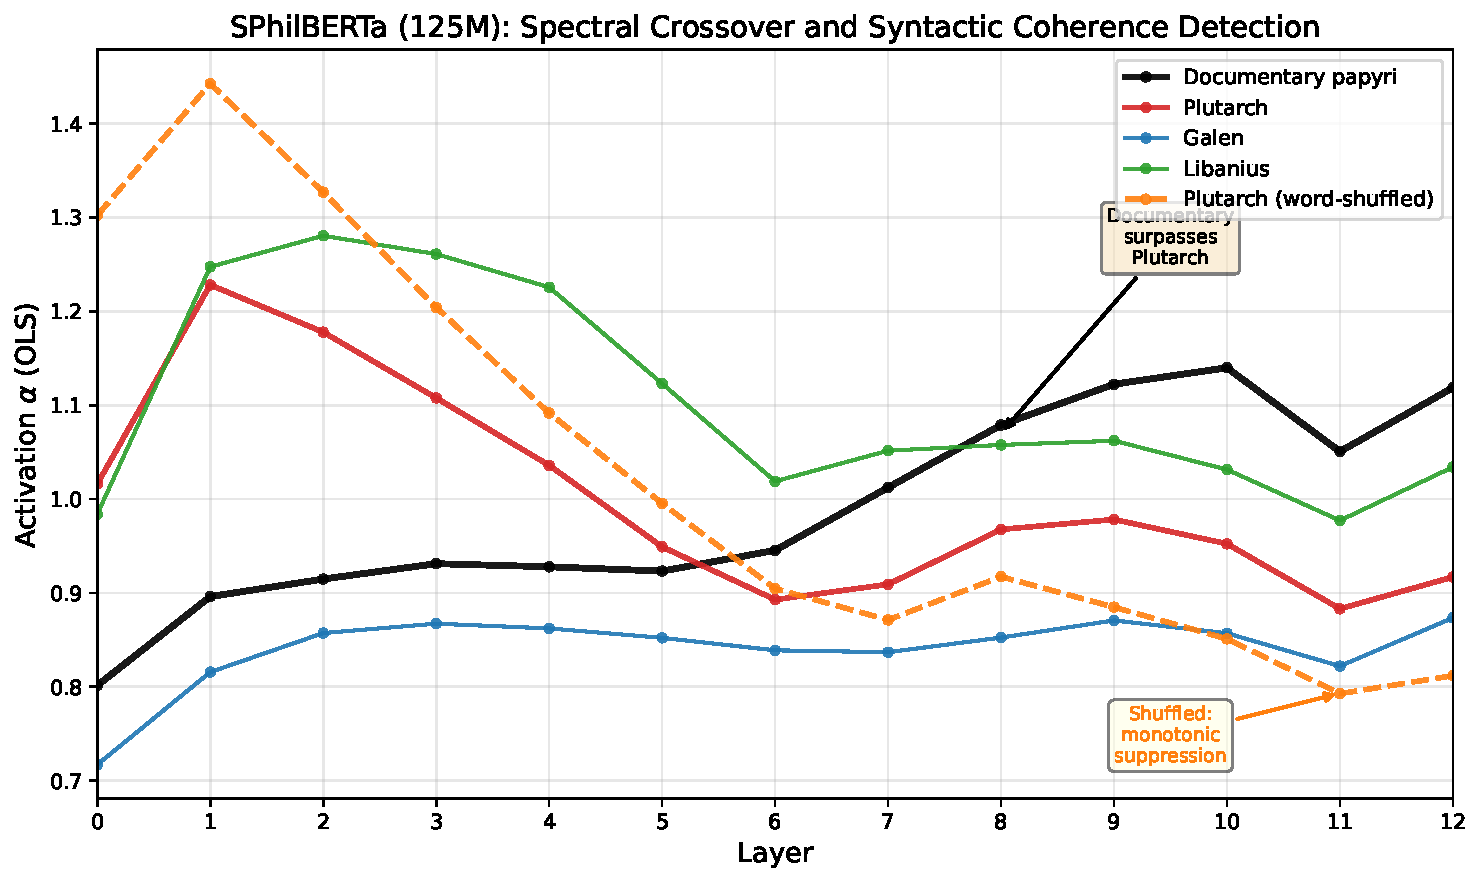
\includegraphics[width=\textwidth]{fig2_sphilberta_crossover.pdf}
\caption{SPhilBERTa activation $\al$ trajectories (13 layers).
Documentary papyri (dark) rise through layers while literary
authors (Plutarch, red) drop---the spectral ordering inverts.
Word-shuffled Plutarch (orange, dashed) drops monotonically,
revealing an implicit syntactic coherence detector.}
\label{fig:sphilberta}
\end{figure}

SPhilBERTa \citep{riemenschneider2023}---a 125M parameter RoBERTa
trained on Ancient Greek and Latin---exhibits a pattern strikingly
different from the generalist models.  In Qwen 72B, input spectral
ordering is passively preserved through all layers: if documentary
starts lowest, it ends lowest.  In SPhilBERTa, the ordering
\emph{inverts}: documentary papyri, which start spectrally simple,
get enriched through layers, while literary text, which starts
spectrally rich, gets compressed.

This is not a side effect.  The specialist model has learned to
\emph{equalize} the spectral complexity of its inputs.  Downstream
tasks (translation search, semantic similarity) are better served by
representations where different registers have comparable spectral
dimensionality, rather than preserving the raw distributional
differences.

Additionally, syntactically destroyed input (word-shuffled Plutarch)
starts with the highest $\al$ at layer 0 ($\al = 1.30$) and drops
through layers to the lowest $\al$ at the output ($\al = 0.81$ at
layer 12, vs.\ unshuffled Plutarch at $0.92$).  Meanwhile,
documentary papyri rise from $\al = 0.80$ at layer 0 to $\al = 1.12$
at layer 12---surpassing Plutarch by layer 8.  SPhilBERTa
progressively removes spectral diversity from input that lacks
syntactic structure while enriching spectrally simple but
syntactically coherent input: an implicit syntactic coherence
detector operating through spectral compression.

\begin{table}[H]
\centering
\caption{SPhilBERTa activation $\al$ through 13 layers
(selected layers).  Shuffled Plutarch drops monotonically;
documentary rises and crosses over literary authors.}
\label{tab:sphilberta}
\begin{tabular}{rrrrrr}
\toprule
\textbf{Layer} & \textbf{Doc.} & \textbf{Plutarch} &
\textbf{Galen} & \textbf{Libanius} & \textbf{Plut.\ shuf.} \\
\midrule
0 & 0.801 & 1.016 & 0.717 & 0.984 & 1.302 \\
3 & 0.931 & 1.108 & 0.867 & 1.261 & 1.204 \\
6 & 0.945 & 0.893 & 0.839 & 1.019 & 0.905 \\
9 & 1.122 & 0.978 & 0.871 & 1.062 & 0.885 \\
12 & 1.119 & 0.917 & 0.873 & 1.034 & 0.812 \\
\bottomrule
\end{tabular}
\end{table}

\subsection{Cross-Model Universality}
\label{sec:crossmodel}

\begin{table}[H]
\centering
\caption{Final-layer activation $\al$ for greek\_documentary and
math.AG across six architectures spanning four families.
Documentary is lowest or near-lowest in every model except the
specialist (SPhilBERTa), which inverts the ordering.}
\label{tab:crossmodel}
\begin{tabular}{llrrrl}
\toprule
\textbf{Model} & \textbf{Architecture} & \textbf{Params} &
\textbf{doc $\al$} & \textbf{math.AG $\al$} & \textbf{Note} \\
\midrule
Qwen 2.5-72B & Dense decoder, GQA & 72B & 0.647 & 0.914 & Lowest \\
Llama 3.3-70B & Dense decoder, GQA & 70B & 0.769 & 1.180 & Lowest \\
Nomic v2 MoE & Encoder + MoE & 475M & 1.104 & 1.272 & Lowest \\
PPLX 0.6B & Encoder (Qwen3) & 596M & 1.854 & 2.714 & Near-lowest \\
PPLX 4B & Encoder (Qwen3) & 4B & 1.914 & 2.524 & Near-lowest \\
SPhilBERTa & Encoder (RoBERTa) & 125M & --- & --- & Inverted \\
\bottomrule
\end{tabular}
\end{table}

Greek documentary text produces the lowest or near-lowest
activation $\al$ at the final layer in every tested model except
SPhilBERTa (which actively inverts the ordering).  The signal is in
the text, not the model.  Across four architecture families (dense
decoder, encoder-only, encoder + MoE, domain specialist), spanning
125M to 72B parameters, the spectral separation of documentary
Koine persists.

\paragraph{Nomic v2 MoE: closing the loop.}  The Nomic v2 MoE
result is particularly significant because Nomic is the model used
to generate the embedding-level $\al$ values throughout this paper.
The fact that documentary $\al$ is lowest at \emph{every layer}
inside Nomic---not just at the output---means the embedding-level
$\al$ divergence between documentary and literary text is consistent
with the per-layer $\al$ divergence inside the model that produced
those embeddings.  The absolute values differ (documentary $\al =
1.104$ at the final internal layer vs.\ $\al = 0.868$ at the
embedding level, Table~\ref{tab:register}) because the two
measurements operate at different $N$, use different matrix
constructions (activation covariance vs.\ embedding-space Gram
matrix), and sample different subsets of the corpus.  But the
rank ordering is consistent: the outer-level measurement and the
inner-level measurement agree on which register is spectrally
simplest.


% ══════════════════════════════════════════════════════════════
\section{Discussion}
\label{sec:discussion}
% ══════════════════════════════════════════════════════════════

\subsection{What $\al$ Measures}

$\al$ measures the effective rank of the content's semantic
covariance matrix, filtered through the model's learned projection.
A corpus of tax receipts concentrates eigenvalue energy in a few
modes because the documents share a small template vocabulary (date,
name, commodity, amount).  Satirical dialogues distribute energy
across many modes because each dialogue inhabits a different semantic
space.  $\al$ is measuring how many independent things the text is
trying to say at once.

This is not a metaphor.  The Gram matrix $G$ is the empirical
covariance of the corpus in embedding space.  Its eigenvalues
quantify the variance explained by each principal component.  A high
$\al$ indicates a slowly decaying eigenvalue tail: many eigenvalues
contribute at each scale, meaning the corpus occupies many
independent semantic dimensions.  A low $\al$ indicates rapid
eigenvalue decay: energy concentrates in a few dominant modes,
reflecting low effective dimensionality.

\subsection{Syntactic Compression as a Measurable Spectral Effect}

The word-shuffle experiment establishes that natural word order
reduces $\al$ by 15--20\% relative to bag-of-words.  This means
syntax creates correlations between semantic modes that would
otherwise be independent.  The resulting decomposition---$\al_{\text{total}} = \al_{\text{lexical}} - \dalpha_{\text{syntactic}}$---is, to our knowledge, novel.  $\al_{\text{lexical}}$ (what survives
word shuffle) captures lexical/semantic content.
$\dalpha_{\text{syntactic}}$ (what word shuffle destroys) captures
the spectral effect of syntactic structure.  Both are directly
measurable.

\subsection{Register as Functional Constraint}

The temporal stability of documentary Koine ($\al = 0.847 \pm 0.007$
across a millennium) tells us that the spectral signature of a
register is determined by its functional constraints, not its
historical period.  Tax receipts have the same spectral structure
whether written under the Ptolemies or the Byzantines because the
functional template---identify parties, specify goods, record
transaction---has not changed.  The eigenvalue tail does not track
dynasty; it tracks how many independent things the text is trying to
say at once.

\subsection{Two-Phase Transformer Processing}

The U-shaped activation $\al$ trajectory with uniform soft rank
recovery reveals a two-phase processing architecture:

\begin{enumerate}
\item \textbf{Compression (layers 0--10):} The network compresses
input into a low-dimensional format.  Most domains collapse to
$\al \approx 0.4$.  This erases content-independent spectral
structure.  (Greek literary text resists this compression, likely
due to tokenization effects; see Section~\ref{sec:trajectories}.)

\item \textbf{Content-dependent expansion (layers 10--70):} The
network re-expands representations in a content-dependent manner.
The same weights, applied to different inputs, produce qualitatively
different spectral trajectories.  math.AG rises steeply;
greek\_documentary stays suppressed; random\_english (no syntactic
structure to preserve) explodes upward.
\end{enumerate}

The compression is lossy in a specific way: it preserves the total
energy distribution (soft rank recovers to $\sim$0.93 uniformly)
but allows the shape of the energy distribution (measured by $\al$)
to vary by content.  The network functions as a spectral filter:
it removes content-independent structure early, and the remaining
computation operates on content-dependent structure.

\subsection{Generalist vs.\ Specialist Spectral Behavior}

The SPhilBERTa crossover (Section~\ref{sec:sphilberta}) is the key
architectural finding.  A generalist (Qwen) passively preserves the
input spectral ordering through all layers: if documentary starts
lowest, it ends lowest.  A specialist (SPhilBERTa) actively inverts
it: documentary gets spectrally enriched, literary gets compressed.
The specialist learned to equalize the spectral complexity of its
inputs as part of its representation learning.

This suggests a testable architectural intervention: adding an
auxiliary loss term during training that penalizes large $\al$
divergence between domains at the output layer.  The SPhilBERTa
crossover is an existence proof that specialist training naturally
produces spectral equalization; the question is whether explicitly
optimizing for it improves cross-register transfer performance.
The $\al$ computation is differentiable (eigendecomposition has
known gradients), so this regularization is implementable without
architectural changes.

\subsection{Limitations}

\begin{enumerate}
\item $\al$ absolute values depend on $N$, $D$, tail fraction $f$,
and estimator.  All comparisons require matched conditions.

\item The LOOCV bimodal accuracy distribution (100\% at extremes,
0\% in middle) reflects the fundamental limitation of a scalar
diagnostic.  $\al$ alone cannot distinguish categories with similar
spectral exponents.

\item Three categories (physics.hist-ph, q-bio.MN, astro-ph.CO)
have weak effect sizes ($z < 3$) in the label shuffle test.  Their
$\al$ separation from the null is statistically significant due to
the high power of 1{,}000 permutations, but practically small.

\item Internal spectroscopy has been performed on six architectures
but not yet on large mixture-of-experts decoders (e.g., DeepSeek R1,
256 experts).  Whether expert routing correlates with spectral
regime is an open question.

\item The greek\_literary anomaly at layer 5 (failure to compress)
requires further investigation.  We attribute it to tokenization
effects (rare polytonic subword tokens in underused embedding
regions), but cannot rule out structural properties of the language
itself.

\item The syntactic compression decomposition
($\dalpha_{\text{syntactic}}$) is demonstrated but not formalized.
A rigorous information-theoretic treatment connecting $\al$ to
mutual information or entropy rate is needed.

\item Small-$N$ results ($N < 20$) are unreliable and should not
be interpreted.

\item One primary embedding model (Nomic v2 MoE) is used
throughout, with cross-validation on five others.
\end{enumerate}


% ══════════════════════════════════════════════════════════════
\section{Conclusion}
\label{sec:conclusion}
% ══════════════════════════════════════════════════════════════

This paper reports a trajectory from falsification to discovery.
A prior analysis attributed domain-discriminative power to the mean
spacing ratio $\rbar$; that claim was false, and the DOI was
withdrawn.  The subsequent investigation established that $\rbar$
measures model geometry while $\al$ measures content structure.

$\al$ diverges across 25 arXiv categories ($p < 0.001$, with $z$-scores
ranging from 0.7 to 26.8), across linguistic registers within
dialect-controlled Koine Greek (documentary 0.87, literary papyri
1.00, literary authors 1.49), and across 20 individual authors
within the same dialect (range 0.72--4.88).  It is temporally stable
across 1{,}000 years of documentary papyri ($\pm 0.01$), robust to
subsampling (CV $= 0.2\%$), and plausible as a power-law exponent
(24/25 categories pass CSN bootstrap).  LOOCV achieves 52.5\%
classification accuracy (13$\times$ chance), with 100\% accuracy at
the extremes of the $\al$ distribution and 0\% in the middle---the
expected behavior of a scalar diagnostic.

Word-order shuffling inflates $\al$ by 15--20\% with zero token
count change, establishing syntactic compression as a measurable
spectral effect and eliminating tokenization artifacts.  Internal
spectroscopy across six architectures (125M--72B parameters)
reveals a two-phase processing pipeline: compression followed by
content-dependent expansion.  Weight $\al$ shows a generally
increasing trend through depth and is domain-independent; activation
$\al$ diverges by content.  A domain-specialist model (SPhilBERTa)
inverts the spectral ordering of its inputs, suggesting that
spectral equalization is a learned property of representation
learning.

The signal is in the text, not the model.  Greek documentary papyri
produce the lowest activation $\al$ across four architecture
families spanning three orders of magnitude in parameter count.
$\al$ fingerprints how many independent things a corpus is trying
to say at once---and that number is determined by functional
constraints, not by historical period, dialect, or model
architecture.

All code and data are available at
\url{https://github.com/spectral-universality/spectral-rmt-pipeline}.


% ══════════════════════════════════════════════════════════════
% References
% ══════════════════════════════════════════════════════════════

\begin{thebibliography}{20}

\bibitem[Marchenko and Pastur(1967)]{marchenko1967}
V.~A. Marchenko and L.~A. Pastur.
\newblock Distribution of eigenvalues for some sets of random matrices.
\newblock \emph{Math. USSR-Sbornik}, 1(4):457--483, 1967.

\bibitem[Oganesyan and Huse(2007)]{oganesyan2007}
V.~Oganesyan and D.~A. Huse.
\newblock Localization of interacting fermions at high temperature.
\newblock \emph{Physical Review B}, 75(15):155111, 2007.

\bibitem[Martin and Mahoney(2021)]{martin2021}
C.~H. Martin and M.~W. Mahoney.
\newblock Implicit self-regularization in deep neural networks: Evidence from
  random matrix theory and implications for training.
\newblock \emph{JMLR}, 22(165):1--63, 2021.

\bibitem[Staats(2024)]{staats2024}
T.~Staats.
\newblock {RMT} analysis of transformer weights.
\newblock arXiv:2410.17770, 2024.

\bibitem[Hayden(2026)]{hayden2026zenodo}
J.~Hayden.
\newblock Spectral universality in embedding similarity matrices.
\newblock Zenodo, 2026.
\newblock (DOI withdrawn after falsification of $\rbar$ results.)

\bibitem[Clauset et~al.(2009)]{clauset2009}
A.~Clauset, C.~R. Shalizi, and M.~E.~J. Newman.
\newblock Power-law distributions in empirical data.
\newblock \emph{SIAM Review}, 51(4):661--703, 2009.

\bibitem[Hill(1975)]{hill1975}
B.~M. Hill.
\newblock A simple general approach to inference about the tail of a
  distribution.
\newblock \emph{Annals of Statistics}, 3(5):1163--1174, 1975.

\bibitem[{papyri.info}(2026)]{papyriinfo}
{Integrating Digital Papyrology}.
\newblock \url{https://papyri.info/}, 2026.

\bibitem[{First1KGreek}(2026)]{first1kgreek}
{First1KGreek Project}.
\newblock \url{https://opengreekandlatin.github.io/First1KGreek/}, 2026.

\bibitem[{Nomic AI}(2024)]{nomic2024}
{Nomic AI}.
\newblock Nomic Embed: Training a reproducible long context text embedder.
\newblock arXiv:2402.01613, 2024.

\bibitem[Riemenschneider and Frank(2023)]{riemenschneider2023}
F.~Riemenschneider and A.~Frank.
\newblock \emph{Graecia capta ferum victorem cepit}.
  {D}etecting {L}atin allusions to {A}ncient {G}reek literature.
\newblock In \emph{Proceedings of the First Workshop on Ancient Language
  Processing (ALP)}, Varna, Bulgaria, 2023.
\newblock arXiv:2308.12008.

\end{thebibliography}


\end{document}
